\documentclass[11pt]{article}
\usepackage{euscript}

\usepackage{amsmath}
\usepackage{amsthm}
\usepackage{amssymb}
\usepackage{epsfig}
\usepackage{xspace}
\usepackage{color}
\usepackage{url}

%%%%%%%  For drawing trees  %%%%%%%%%
\usepackage{tikz}
\usetikzlibrary{calc, shapes, backgrounds}

%%%%%%%%%%%%%%%%%%%%%%%%%%%%%%%%%
\setlength{\textheight}{9in}
\setlength{\topmargin}{-0.600in}
\setlength{\headheight}{0.2in}
\setlength{\headsep}{0.250in}
\setlength{\footskip}{0.5in}
\flushbottom
\setlength{\textwidth}{6.5in}
\setlength{\oddsidemargin}{0in}
\setlength{\evensidemargin}{0in}
\setlength{\columnsep}{2pc}
\setlength{\parindent}{1em}
%%%%%%%%%%%%%%%%%%%%%%%%%%%%%%%%%


\newcommand{\eps}{\varepsilon}

\renewcommand{\c}[1]{\ensuremath{\EuScript{#1}}}
\renewcommand{\b}[1]{\ensuremath{\mathbb{#1}}}
\newcommand{\s}[1]{\textsf{#1}}

\newcommand{\E}{\textbf{\textsf{E}}}
\renewcommand{\Pr}{\textbf{\textsf{Pr}}}

\title{Homework Form for Probability and Statistics for Engineers
\footnote{\s{CS 3130 / ECE 3530 ProbStats; \;\; Fall 2014 \hfill
Instructor: Jeff M. Phillips, University of Utah}
}
}
\author{Your name goes here}

\begin{document}
\maketitle





%%%%%%%%%%%%%%%%%%%%%%%%%%%%%%%%%%%%%%%%%%%%%%%%%%%%
%%%%%%%%%%%%%%%%%%%%%%%%%%%%%%%%%%%%%%%%%%%%%%%%%%%%
%%%%%%%%%%%%%%%%%%%%%%%%%%%%%%%%%%%%%%%%%%%%%%%%%%%%
\section{Overview}

This is a sample latex file to use for completing assignments.  This particular file is not required.  In fact, there are many cool ways to spruce up this plain look.  Feel free to use them.  

\section{Clarity}
I recommend you number sections according to the homework questions and subquestions.  This will make grading very easy, and make it less likely that your answers will be misinterpreted.  There is no text required outside these areas.  

For subquestions, you can use either enumerated lists:
\begin{enumerate}
\item This little piggy went to market,
\item This little piggy stayed home,
\item This little piggy had roast beef,
\item This little piggy had none,
\item And this little piggy cried wee wee wee all the way home.
\end{enumerate}
to itemized lists:
\begin{itemize}
\item mama bear
\item papa bear
\item baby bear.  
\end{itemize}


\section{Figures}
Figures are very easy in Latex.  See the example below:

\begin{figure}[h]
\centering{
\includegraphics[width=.6\linewidth]{figurefilepath.pdf}
}
\caption{Add an optimal caption.}
\label{fig:name}
\end{figure}

The text in the \s{label} command allows one to refer to the Figure number, in this case I am referring to Figure \ref{fig:name}.  

\section{Macros}
I have included a few simple macros at the top.  For instance use $\Pr[X]$ to indicate the probability of $X$ and use $\E[X]$ to refer to the expected value of $X$.  I usually use a script font $\c{X}$ to refer to a set, for instance $\c{X} = \{X_1, X_2, \ldots, X_n\}$ may indicate a set of $n$ random variables.  

There are lots of other neat math macros built into Latex.  Use dollar signs (e.g. $X_i$) to offset some math text and use slash brackets 
\[
M = \sum_{i=1}^n X_i
\]
to use an entire line to write a longer expression.  

For set notation it useful to use
\begin{itemize}
\item $A$ is the set of numbers $\{1, 2, 4, 6, 3\}$.
\item $A \subseteq B = \{1,2,3,4,5,6\}$
\item intersection of $A$ and $B$ as $A \cap B$
\item union of $A$ and $B$ as $A \cup B$
\item an element of a set $x \in A$
\item events $(x,y) \in X \times Y$.  
\item and the reals $\mathbb{R}$, integers $\mathbb{Z}$, rationals $\mathbb{Q}$.  
\end{itemize}


\section{Drawing Trees in Latex}
This section uses the tikz package.  It shows how to draw a basic probability tree corresponding to the ones in the notes for lecture L02.  Its not quite as pretty, but is done entirely within Latex.  

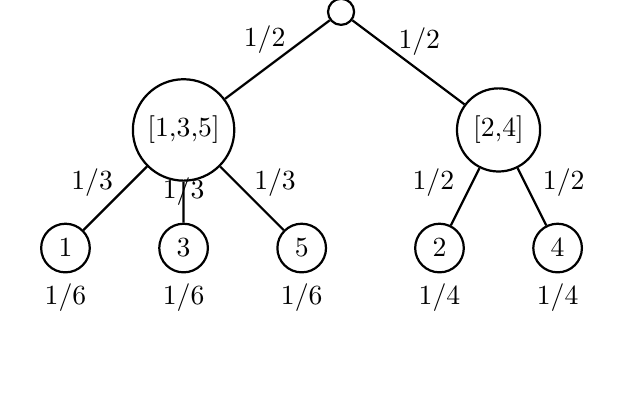
\begin{tikzpicture}[
    scale = 1, transform shape, thick,
    every node/.style = {draw, circle},
    grow = down,  % alignment of characters
    level 1/.style = {sibling distance=4cm},
    level 2/.style = {sibling distance=1.5cm}, 
    level distance = 1.5cm
  ]
  \node (Start) {} 
   child {   node (A) {[1,3,5]}
     child { node (B) {1}}
     child { node (C) {3}}
     child { node (D) {5}}
   }
   child {   node (E) {[2,4]}
     child { node (F) {2}}
     child { node (G) {4}}
   };


  % Put probability on edges
  \begin{scope}[nodes = {draw = none}]
    \path (Start) -- (A) node [near start, left]  {$1/2$};
    \path (A)     -- (B) node [near start, left]  {$1/3$};
    \path (A)     -- (C) node [near start] {$1/3$};
    \path (A)     -- (D) node [near start, right] {$1/3$};
    \path (Start) -- (E) node [near start, right] {$1/2$};
    \path (E)     -- (F) node [near start, left]  {$1/2$};
    \path (E)     -- (G) node [near start, right] {$1/2$};
    \begin{scope}[nodes = {below = 4pt}]
      \node at (B) {$1/6$};
      \node at (C) {$1/6$};
      \node at (D) {$1/6$};
      \node at (F) {$1/4$};
      \node at (G) {$1/4$};
    \end{scope}
  \end{scope}
\end{tikzpicture}



\section{More help}
Latex has gotten quite popular, so much so that if you type ``latex'' into google, it lists nothing on the first page about gloves.  

There are some great free references already out there for instance:
\begin{itemize}
\item \url{http://en.wikibooks.org/wiki/LaTeX}
\item \url{http://tex.stackexchange.com/}
\end{itemize}

\end{document}
